\documentclass[tikz,border=5pt]{standalone}
\usepackage{tikz}
\usepackage{amsmath}
\usetikzlibrary{arrows.meta,positioning,calc}
\definecolor{nebula}{HTML}{6366F1}
\definecolor{spark}{HTML}{14B8A6}
\definecolor{ink}{HTML}{334155}
\begin{document}
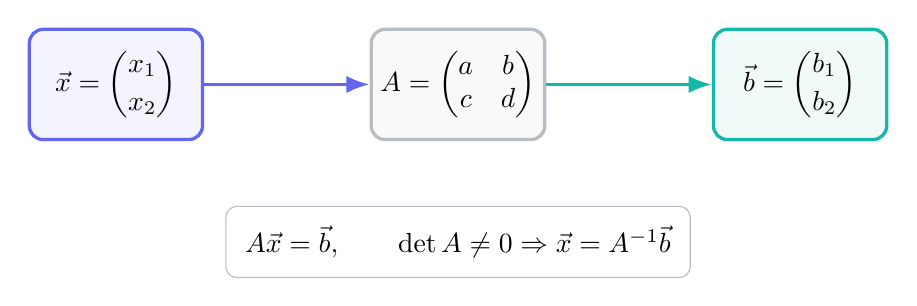
\begin{tikzpicture}[font=\sffamily,>=Latex,node distance=2.1cm]
  \tikzset{box/.style={draw=ink!35,rounded corners=5pt,very thick,fill=white,minimum height=1.4cm,minimum width=2.2cm,align=center}}
  \node[box,draw=nebula,fill=nebula!7] (x) {$\displaystyle \vec x=\binom{x_1}{x_2}$};
  \node[box,right=of x,fill=ink!3] (a) {$\displaystyle A=\begin{pmatrix}a&b\\c&d\end{pmatrix}$};
  \node[box,right=of a,draw=spark,fill=spark!7] (b) {$\displaystyle \vec b=\binom{b_1}{b_2}$};
  \draw[->,very thick,nebula] (x)--(a);
  \draw[->,very thick,spark] (a)--(b);
  \node[draw=ink!35,rounded corners=4pt,fill=white,inner sep=7pt] at ($(a)+(0,-2.0)$)
    {$A\vec x=\vec b,\qquad \det A\neq0\Rightarrow \vec x=A^{-1}\vec b$};
\end{tikzpicture}
\end{document}
